% Created 2019-12-02 月 17:36
\documentclass{article}
\usepackage[utf8]{inputenc}
\usepackage[T1]{fontenc}
\usepackage{fixltx2e}
\usepackage{graphicx}
\usepackage{longtable}
\usepackage{float}
\usepackage{wrapfig}
\usepackage{rotating}
\usepackage[normalem]{ulem}
\usepackage{amsmath}
\usepackage{textcomp}
\usepackage{marvosym}
\usepackage{wasysym}
\usepackage{amssymb}
\usepackage{hyperref}
\tolerance=1000
\usepackage[margin=1.0in]{geometry}
\usepackage{mymacros}
\author{hisanobu-nakamura}
\date{\textit{<2019-11-20 水>}}
\title{Cassinian Cookies}
\hypersetup{
  pdfkeywords={},
  pdfsubject={},
  pdfcreator={Emacs 25.3.2 (Org mode 8.2.10)}}
\begin{document}

\maketitle
\tableofcontents


\section{Generalized Cassinian Curves, Surfaces and Hypersurfaces}
\label{sec-1}
\subsection{The Curves of Cassini in 2D Plane}
\label{sec-1-1}
\begin{figure}[h]
\begin{center}
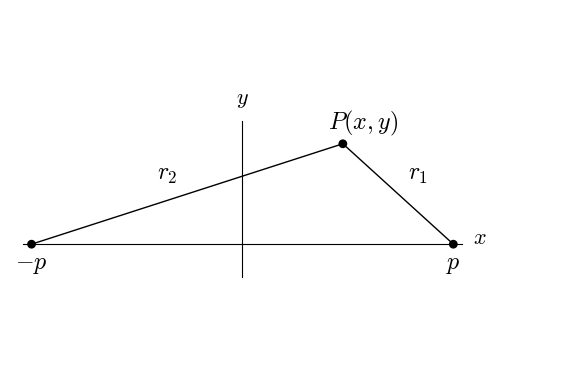
\includegraphics[width=6cm]{cassini_generic_point.png}
\caption{}
\label{ }
\end{center}
\end{figure}
The \emph{curves of Cassini}, or \emph{Cassinian curevs}, in $\R^2$ are defined as follows: given two poins $p_1, p_2 \in \R^2$, called focus, and a real number $a \in \R$, 
the Cassinian curve with the focses $p_{1},p_{2}$ is the set of points $x \in \R^2$ whose product of the Euclidean distances $r_i = \sqrt{|x-p_i|}, \; (i=1,2)$ are always constant $a^2$:
\begin{equation}
\label{ }
r_1 r_2 = a^2.
\end{equation}
They were first introduced by Cassini as orbits of the heavenly bodies, but later discarded as a physical model for astrophysics.
\begin{figure}[h]
\begin{center}
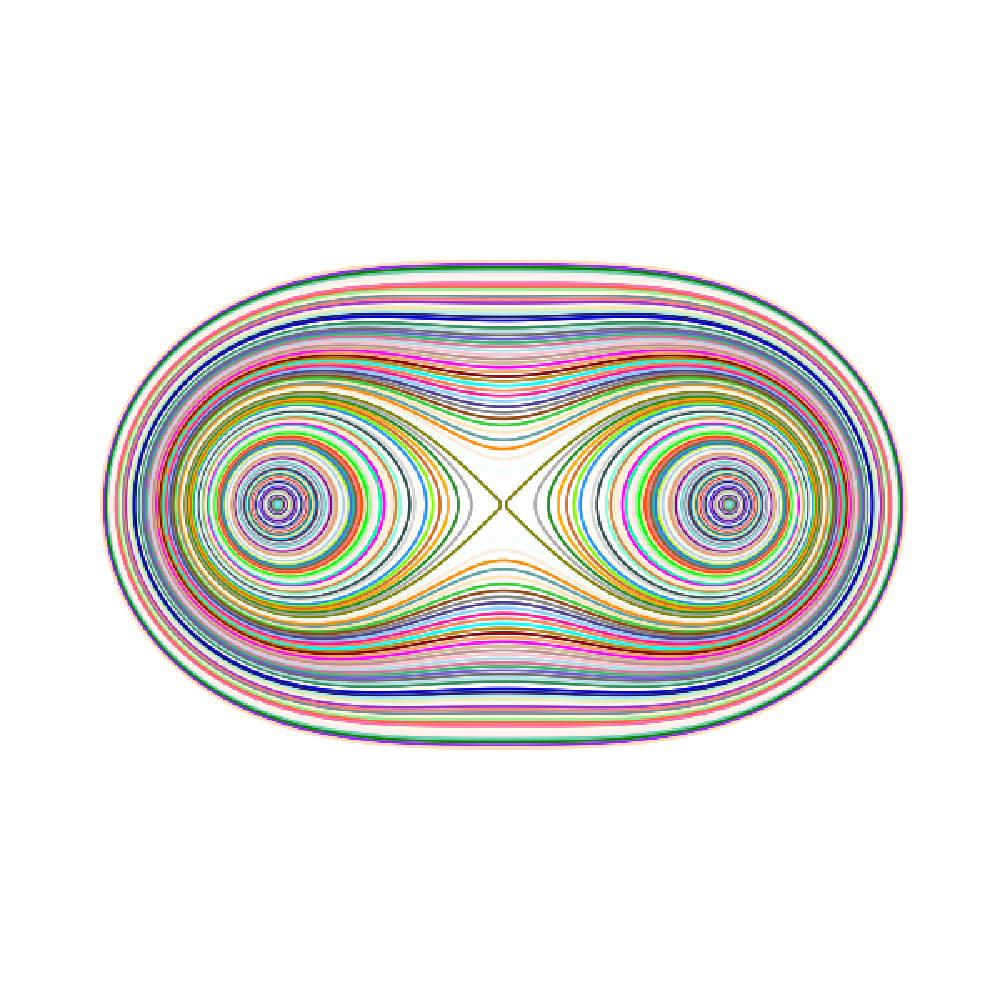
\includegraphics[width=6cm]{cassini2.eps}
\caption{Cassinian curves with varying parameter $a$}
\label{ }
\end{center}
\end{figure}
\subsection{Generalisations}
\label{sec-1-2}
There are two immediate generalisations of the definition of Cassinian curves: (i) increase the number $n$ of foci or/and (ii) increase the dimensionality $D$ of the ambient space $\R^{D}$. 
Let us denote a generic point in the ambient space $\R^{D}$ by $x =(x^1, x^2, \cdots, x^D)$, $n$ distinct fixed points by $p_i \in \R^D, \; (i=1,\cdots, n)$ 
and the values of the distances by $r_i := |x-p_i|$, where $|x|$ is the usual $D$-dimensional Euclidean distance.
 Then define 
\begin{equation}
\label{}
F(p_1,\cdots,p_n;x):=\prod_{i=1}^{n} r_i.
\end{equation}
(D-1)-dimensional Cassinian hypersurface associated with $p_i$'s is defined as the set of points $x\in \R^D$, the product of whose distances from $x$ is equal to a constant $a^2$:
\begin{equation}
\label{ }
C(p_1,\cdots,p_n;a) :=\defset{x\in \R^D}{F(p_1,\cdots,p_n;x) = a^2 }.
\end{equation}
We will often use the abbreviation, $C(P;a)=C(p_1,\cdots,p_n;a)$ in the sequel. 
A further generalisation with arbitrary exponentials can be carried out to obtain \emph{the weighted n-Cassinian curves}, which are defined by:
\begin{eqnarray}
F(P;k;x) & := & \prod_{i=1}^{n} r_i^{k_i} \nonumber\\
C(P;k;a) &:=&\defset{x\in \R^D}{F(P;k;x) = a^2 }
\end{eqnarray}
An example of a weighted Cassinian curve is illustrated in Figure \ref{fig:weited_2_cass}.
%--- DIAGRAM: weighted 2-cassinian ---%
\begin{figure}[h]
\begin{center}
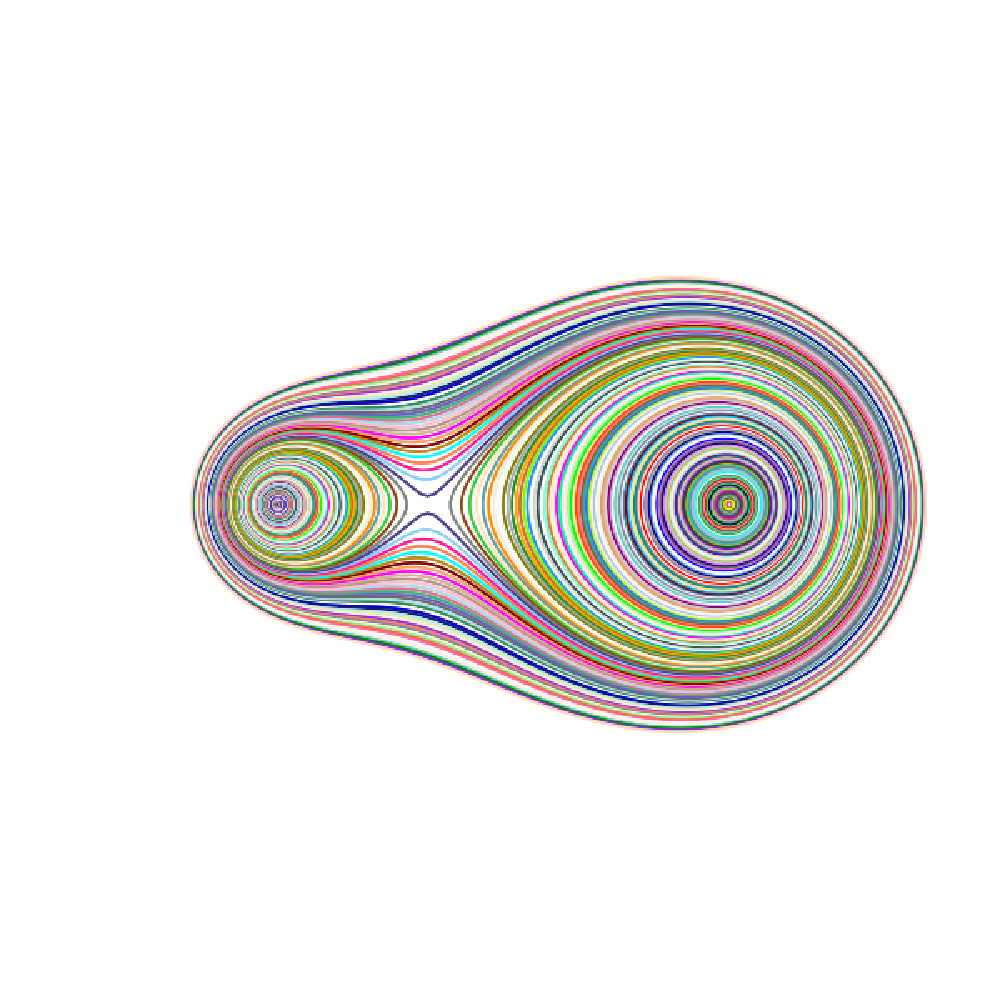
\includegraphics[width=6cm]{cassini2_weighted.eps}
\caption{Weighted 2-Cassinian curve: $r_1 r_2^2 = a^2$}
\label{fig:weited_2_cass}
\end{center}
\end{figure}
However, in this article, we will concentrate mainly on the case $k_i = 1, \forall i$.

When $n=2$, we can assume that $p_1 = (p,0,\dots,0)$ and $p_2 = (-p,0,\dots,0)$ without loss of generality. Then
\begin{equation}
\label{ }
r_1r_2 = \sqrt{(x^1-p)^2 + (x^2)^2 + \cdots + (x^D)^2}\sqrt{(x^1+p)^2 + (x^2)^2 + \cdots + (x^D)^2} = \sqrt{(x^1-p)^2 + R^2}\sqrt{(x^1+p)^2 + R^2}
\end{equation}
with $R^2 = (x^2)^2 + \cdots + (x^D)^2$. Hence, ($D-1$)-dimensional Cassinian hypersurface with two foci is like a lemniscate with its $y$-axes replaced by a $(D-2)$-sphere $S_R^{D-2}$ of radius $R$.

\subsection{Polar Coordinates and Compatibility Conditions}
\label{sec-1-3}
We can compose a list of the data $r_i := |x-p_i|$ and think of the list $(r_1,\cdots,r_n)$ as a point in $\R^n$. 
We call $(r_1,\cdots,r_n)$ \emph{the multipolar coordinates} of the point $x$. 
Every point $x \in \R^D$ has a correspondence in the multipolar coordinate space $\R^n$ defining a map $\phi:\R^D \rightarrow \R^n$. 
When $D>n$, $\phi$ is not surjective, so a point in $\R^n$ corresponds to a $(D-n)$-dimensional hypersurface in $\R^{D}$. 
When $D=n$, a point $r \in (r_1, \cdots,r_n)$ specifies two points in $\R^D$ which are symmetrical about the hyperplane containing the foci $p_i \;(i=1,\cdots,D)$. 
When $D<n$, the image $\phi(\R^D) \subset \R^n$ is a $D$-dimensional hypersurface, which can be specified by some polynomials in $r_i$ and $r_{ij}:=|p_{i}-p_{j}|$. 
Let us call those polynomials compatibility conditions. Usually, we can construct such expressions more than required, so we need to choose out some suitable set of independent ones. 
Once such a set of equations are chosen, they define a $D$ dimensional surface $S$ in $n$-tuple polar coordinate space $r_1:\cdots:r_n \in \R_{pol}^n$, which represents the points in the original Euclidean space $\R^D$. 
Then, if we also plot a surface $C(P;a)$ defined by $r_1\cdots r_n = a^2$ in the multipolar space $\R_{pol}^n$, the intersection $C(P;a) \cap S$ is the set corresponding to a Cassinian surface and for sufficiently small $a$, there are several disconnected components in general. 
Observations in 2 and 3 dimensional spaces tell us that there seem to be $n-1$ disconnected components with $n$ foci in $D=2$ but $n$ components for certain values of $a$ in 3 dimensional space. 
We have not figured out how it really works yet. So, the followings are some observations in low dimensions for small $n$.

\subsection{The 2D Plane Case}
\label{sec-1-4}
First, let us consider the case $D=2$. For $n=2$, the bipolar coordinates $r_1 :r_2$ with $|p_1 -p_2| =2p$ have to satisfy the compatibility conditions, which are, in this case, just triangle inequalities,
\begin{eqnarray}
 r_1 + r_2 & \ge & 2p \\
 r_1 +2p  & \ge & r_2  \\
 r_2 +2p  & \ge & r_1 .
\end{eqnarray}
Here, there is no redundancy. Hence, we only have inequalities, which result in a 2-dimensional region in $\R^2$, the bipolar coordinates plane.
%%% FIGURE: for 2Cassinian %%%
\begin{figure}[h]
\begin{center}
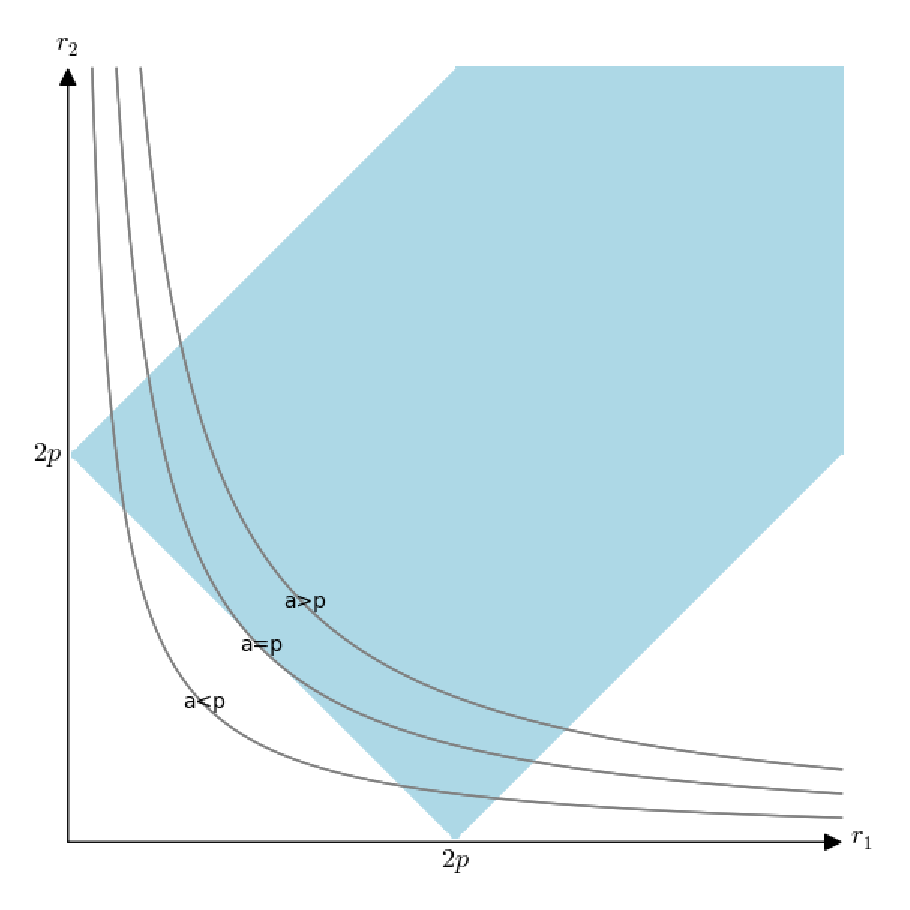
\includegraphics[width=6cm]{2cass_bipo.eps}
\caption{The diagram for the reality region and the cassinian $r_1r_2=a^2$ in bipolar coordinates. Only the portions of the curves intersecting with the shaded region are realised in $\R^2$}
\label{ }
\end{center}
\end{figure}
Note that the boudary of the shaded region corresponds to the line joining the two foci in the original Euclidean plane. Writing $r_{12}=|p_1 -p_2|$, this condition can be written symmetrically as
\begin{equation}
\label{}
( r_1 + r_2 + r_{12})(r_1 + r_2 - r_{12})(r_1 - r_2 + r_{12})(-r_1 + r_2 + r_{12}) = 0.
\end{equation}
This is actually proportional to the square of area as l.h.s. is the inside of the square root of the Heron's formula. We can generalise this inequality to higher dimensions by using a formula by Cayley
\begin{equation}
\label{}
W_2(r_1,r_2;r_{12}) :=   \left|
\begin{array}{cccc}
0 &  r_1^2 & r_2^2 & 1 \\
r_1^2 & 0 & r_{12}^2 & 1\\
r_2^2 & r_{12}^2 & 0 & 1 \\
1 & 1 & 1 & 0
\end{array}\right|=0
\end{equation}
For the case $n=3$, the situation becomes already a bit messy, but there are some useful results known from the classical times. Using the cosine rule for angles $\alpha = \angle BxC, \beta =\angle CxA, \gamma = \angle AxB$, 
\begin{eqnarray}
f_{23} & := & r_2^2 + r_3^2 - r_{23}^2 = 2r_2r_3\cos{\alpha}\\
f_{31} & := & r_3^2 + r_1^2 - r_{31}^2 = 2r_1r_3\cos{\beta}\\
f_{12} & := & r_1^2 + r_2^2 - r_{12}^2 = 2r_1r_2\cos{\gamma}\\
f_{123} & := & r_1^2 r_2^2 r_3^2,
\end{eqnarray}
where $r_{ij}:=|p_i-p_j|$ and the fact that $\alpha + \beta + \gamma = 2\pi$ to eliminate cosines, we obtain the compatibility condition for the tripolars;
\begin{equation}
\label{eq:tri_compat}
F_3(r_1,r_2,r_3;r_{12},r_{23},r_{31}) := f_{23}^2 r_1^2 + f_{31}^2 r_2^2 + f_{12}^2 r_3^2 - 4 f_{123} - f_{23} f_{31} f_{12} = 0.
\end{equation}

Figure \ref{fig:compat_tripol} shows a plot of the compatibility surface in the tripolar coordinates space. Note also that the region inside the purple surface corresponds to two points symmetric in the plane which contains the three foci in the original Euclidean 3 dimensional space. \\
The above compatibility condition can also be stated geometrically: the volume of the tetrahedron formed with the 4 points $p, p_1, p_2, p_3$ is zero i.e. they are coplanar. 
\begin{equation}
\label{}
W_3(r_1,r_2,r_3;r_{12},r_{23},r_{31}) =\left|\begin{array}{ccccc}
0 &  r_{1}^2 & r_{2}^2 & r_{3}^2 & 1 \\
r_{1}^2 &  0 & r_{12}^2 & r_{13}^2 & 1 \\
r_{2}^2 &  r_{21}^2 & 0 & r_{23}^2 & 1 \\
r_{3}^2 &  r_{31}^2 & r_{32}^2 & 0 & 1 \\
 1 & 1 & 1 & 1 & 0  
\end{array}\right|=0
\end{equation} 
%---FIGURE:compatibility surface for a triangle---%
\begin{figure}[H]
\begin{center}
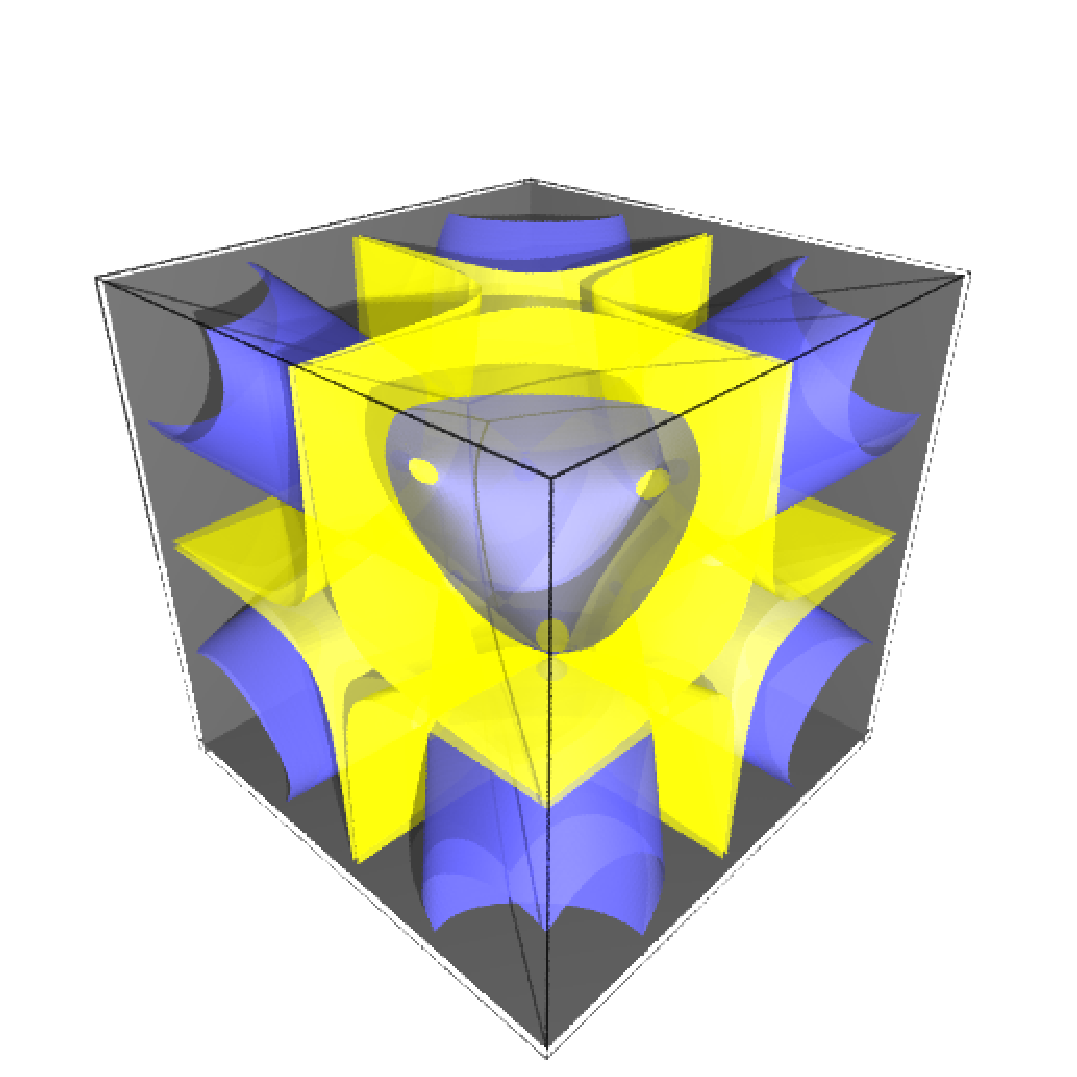
\includegraphics[width=6cm]{compatibility_tripolar.eps}
\caption{A plot of the compatibility surface (purple) for a triangle in tripolar coordinates and the surface (yellow) of points on cassinian curves . Only one sector is valid, but all of them are shown for the visual purpose.}
\label{fig:compat_tripol}
\end{center}
\end{figure}
For $n=4$ or quadrilateral case, the compatibility condition can be expressed as a pair of simultaneous equations. For example, if we calculate one of the diagonal length $l_1$, then we have two compatibility conditions for the two triangles
\begin{eqnarray}
F_3(r_1,r_2,r_3)  & = & F_3(r_2,r_3,r_4)   =  0   
\end{eqnarray}
And then other two relations which involve the other diagonal must be redundant.

In general, compatibility conditions for $n \ge 3$ points $p_i, (i=1,\cdots,n)$ can be written as
\begin{equation}
\label{}
F_3(r_1,r_2,r_3) =  F_3(r_2,r_3,r_4) = \cdots = F_3(r_{n-3},r_{n-2},r_{n-1})= F_3(r_{n-2},r_{n-1},r_{n})=0
\end{equation}

\subsection{The Case in 3D}
\label{sec-1-5}
 When $D=3$, in the cases $n=2$ and $n=3$, the singularities appear in the plane where the focuses lie. 
So the first non-trivial appearance of the singularities occurs when we have $n=4$ non-coplanar foci, which can be seen as the vertices of a tetrahedron. 
Th analogy with triangle will lead us to the similar argument for the construction of the compatibility condition for the quadripolar coordinates. 
That is to divide the tetrahedron $\triangle ABCD$ into four sub-tetrahedra $\triangle xABC$, $\triangle xACD$, $\triangle xABD$ and $\triangle xBCD$ and calculate the solid angles subtended by the vertex $x$, and then eliminate them by using the condition that they must sum up to $4\pi$. 
But we are not going to use this rather naive method here. Instead, we resort to the Cayley determinant for the pentachoron.
\begin{equation}
\label{eq:vol_det}
W_4=
\left|\begin{array}{cccccc}
0 & r_{1}^2 & r_{2}^2 & r_{3}^2 & r_{4}^2 & 1 \\
r_{1}^2 & 0 & r_{12}^2 & r_{13}^2 & r_{14}^2 & 1 \\
r_{2}^2 & r_{21}^2 & 0 & r_{23}^2 & r_{24}^2 & 1 \\
r_{3}^2 & r_{31}^2 & r_{32}^2 & 0 & r_{34}^2 & 1 \\
r_{4}^2 & r_{41}^2 & r_{42}^2 & r_{43}^2 & 0 & 1 \\
1 & 1 & 1 & 1 & 1 & 0  
\end{array}\right|
=0
\end{equation}
\subsubsection{Examples}
\label{sec-1-5-1}
The graphs of some particular Cassinian curves with varying parameter $a$ are listed below. The images were created by using Sage graphics plot.\\
%%-----  3-Casinnians ---%%
\begin{exa}
 Figure \ref{3_cassini_omu} : $ p_1=(0,1), \; p_2 = (-\frac{\sqrt{3}}{2},-\frac{1}{2}), \; p_3 = (\frac{\sqrt{3}}{2},-\frac{1}{2})$\\
Figure \ref{3_cassini_align} : $p_1=(-1,0), \; p_2 = (0,0), \; p_3 = (1,0)$
 %--- DIAGRAMS: third cassinians ---%
\begin{figure}[H]
 %------- Omusubi 3-Cassinian -------%
\begin{minipage}{0.5\hsize}
\begin{center}
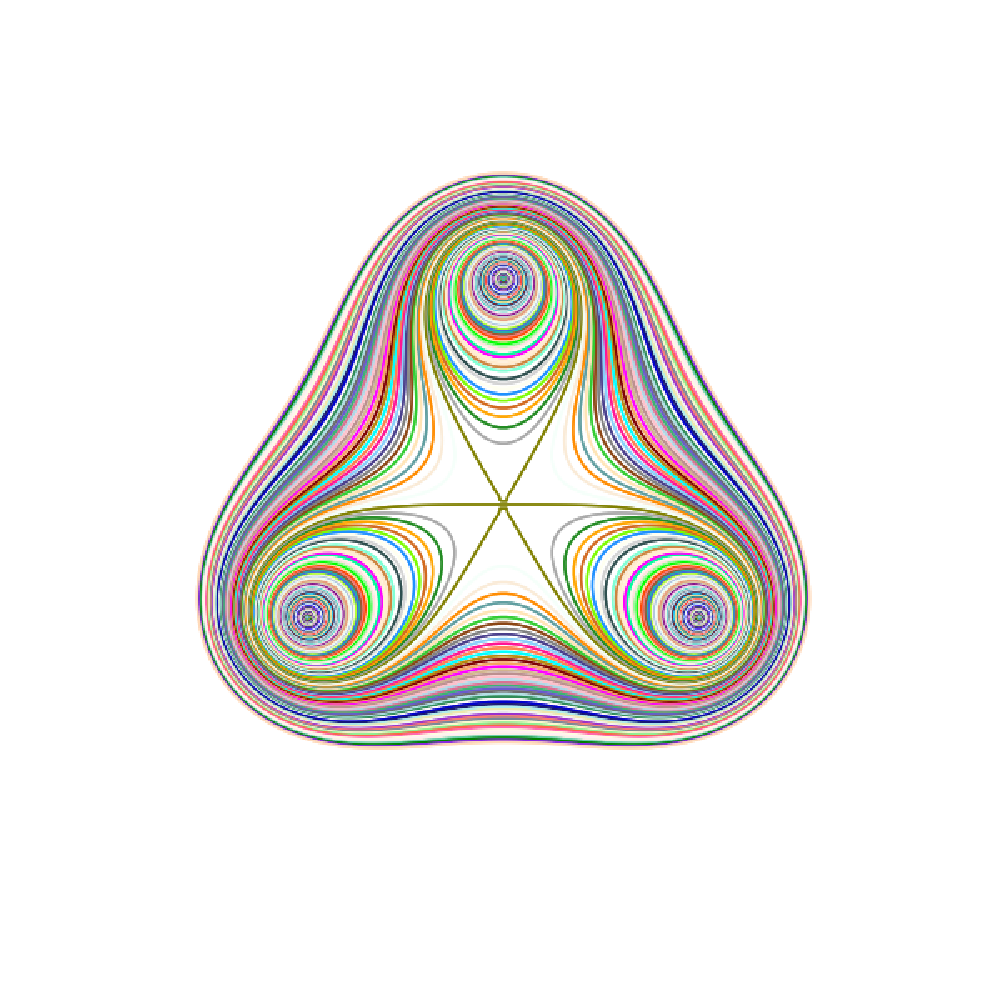
\includegraphics[width=6cm]{cassini3_omusubi.eps}
\caption{}
\label{3_cassini_omu}
\end{center}
\end{minipage}
%------- Aligned 3-Cassinian -------%
\begin{minipage}{0.5\hsize}
\begin{center}
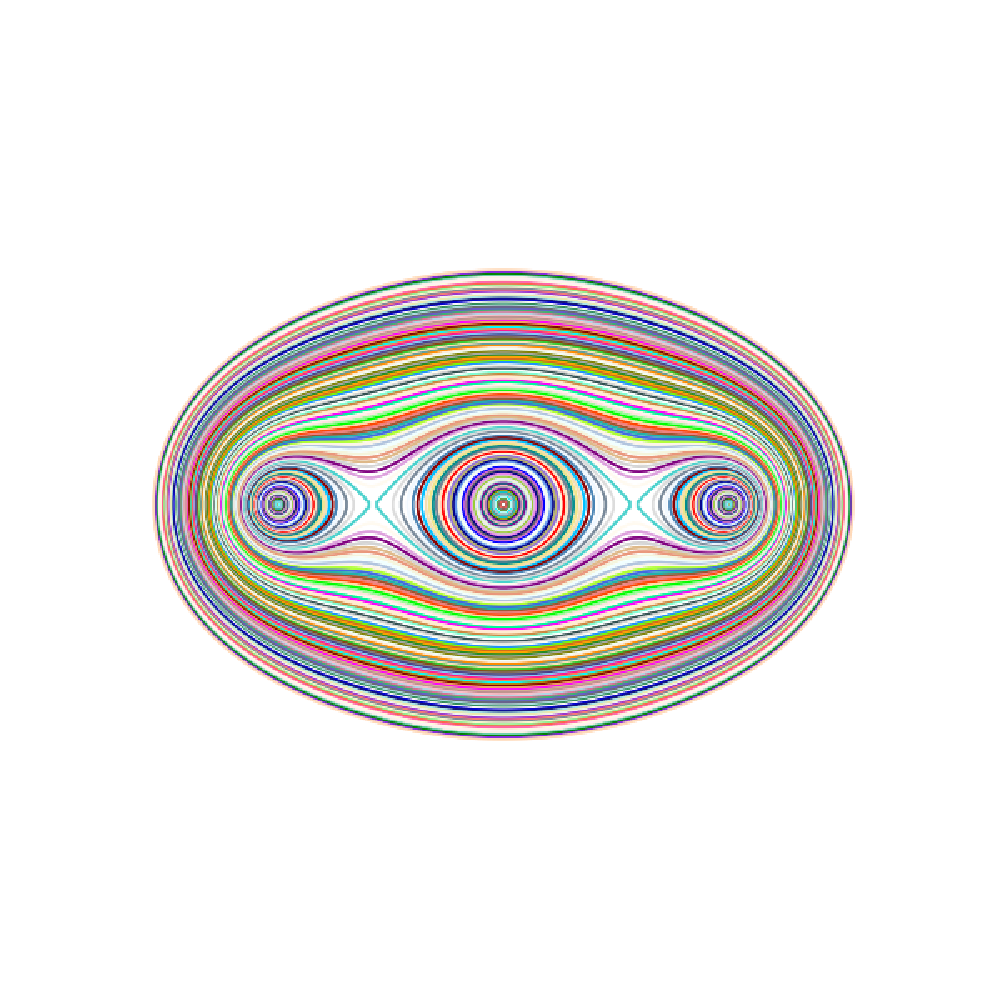
\includegraphics[width=6cm]{cassini3_aligned.eps}
\caption{}
\label{3_cassini_align}
\end{center}
\end{minipage}
\end{figure}
\end{exa}
%% ----  4-Cassinians ---%%
\begin{exa}
\begin{figure}[H]
 %------- Omusubi 4-Cassinian -------%
\begin{minipage}{0.5\hsize}
\begin{center}
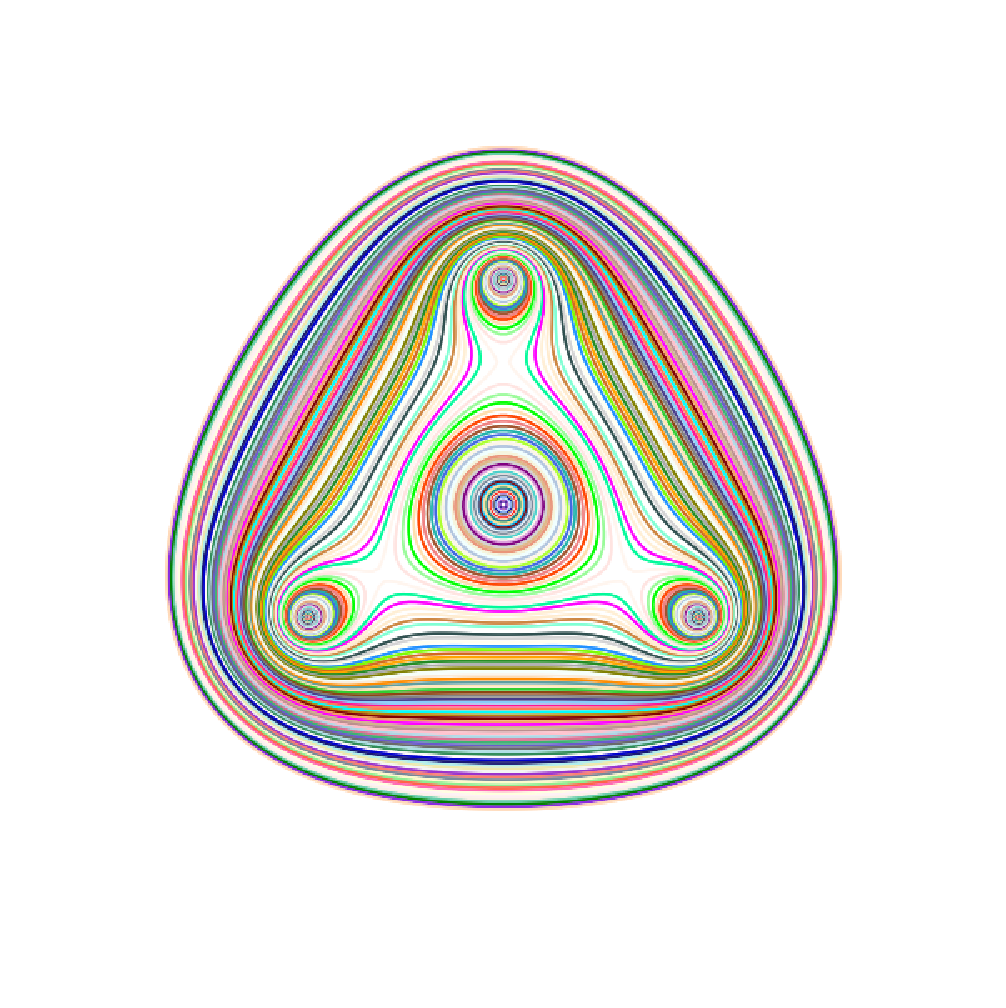
\includegraphics[width=6cm]{cassini4_omusubi.eps}
\caption{}
\label{ }
\end{center}
\end{minipage}
%------- Aligned 4-Cassinian -------%
\begin{minipage}{0.5\hsize}
\begin{center}
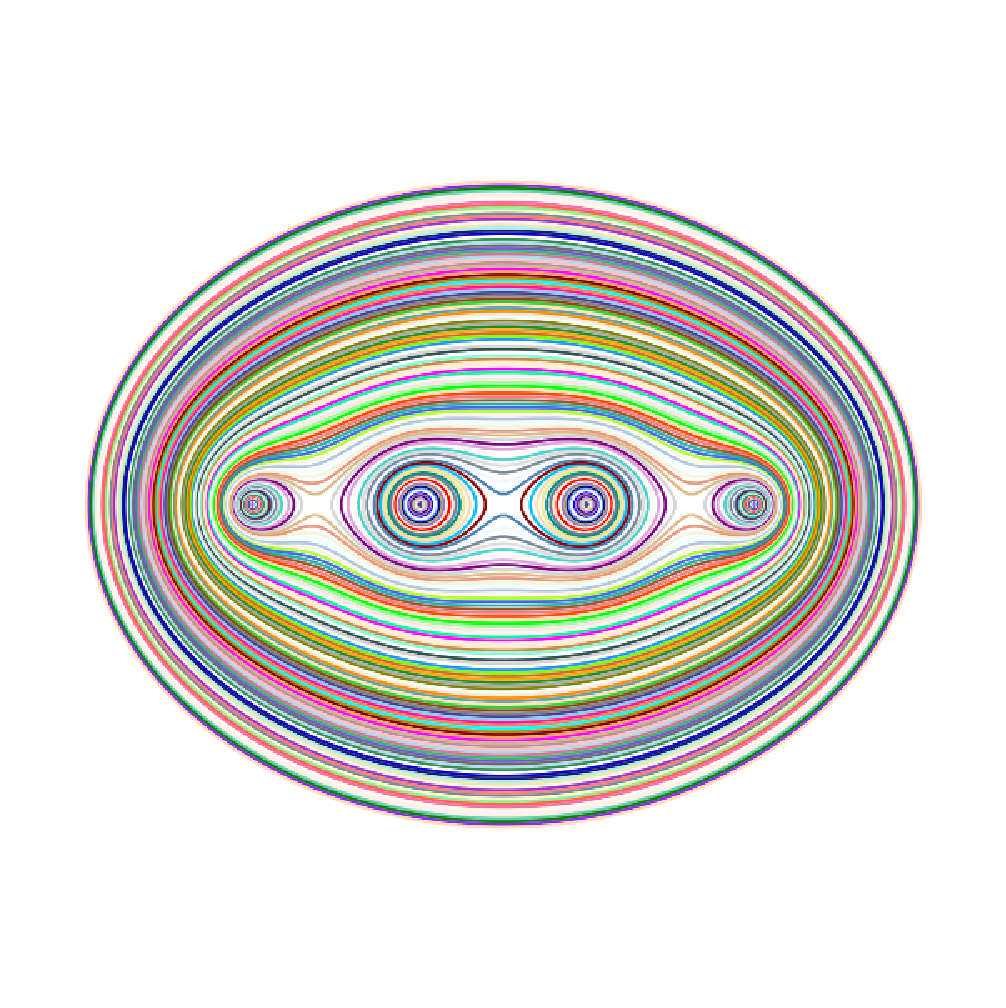
\includegraphics[width=6cm]{cassini4_aligned.eps}
\caption{}
\label{ }
\end{center}
\end{minipage}
\end{figure}
%------- Clover 4-Cassinian -------%
\begin{figure}[H]
\begin{center}
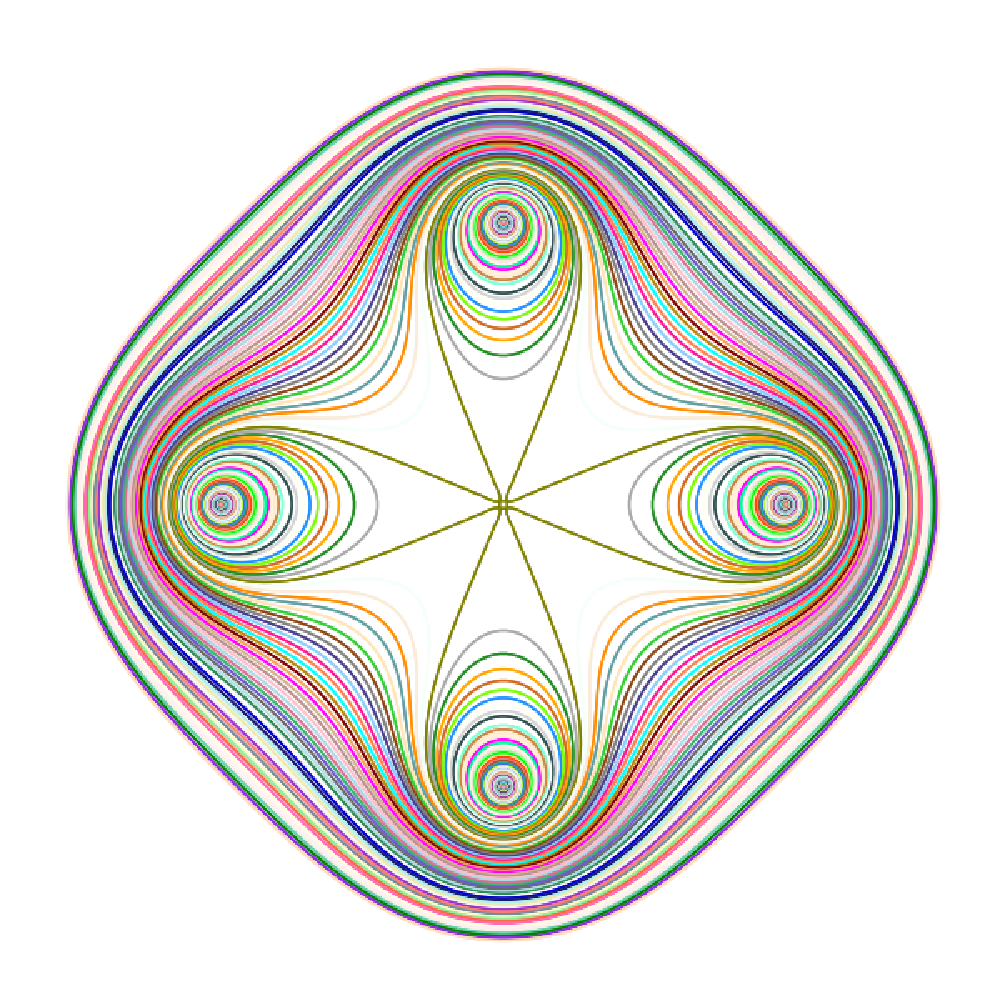
\includegraphics[width=6cm]{cassini4_clover.eps}
\caption{}
\label{ }
\end{center}
\end{figure}
\end{exa}
%% ----  5-Cassinians ---%%
\begin{exa}
$p_1 =(0,1), p_2=(-\sin{\frac{2}{5}\pi},\cos{\frac{2}{5}\pi}), p_3=(-\sin{\frac{4}{5}\pi},\cos{\frac{4}{5}\pi}), p_4=(\sin{\frac{4}{5}\pi},\cos{\frac{4}{5}\pi}), p_5=(\sin{\frac{2}{5}\pi},\cos{\frac{2}{5}\pi})$
%------- Star 5-Cassinian -------%
\begin{figure}[H]
\begin{center}
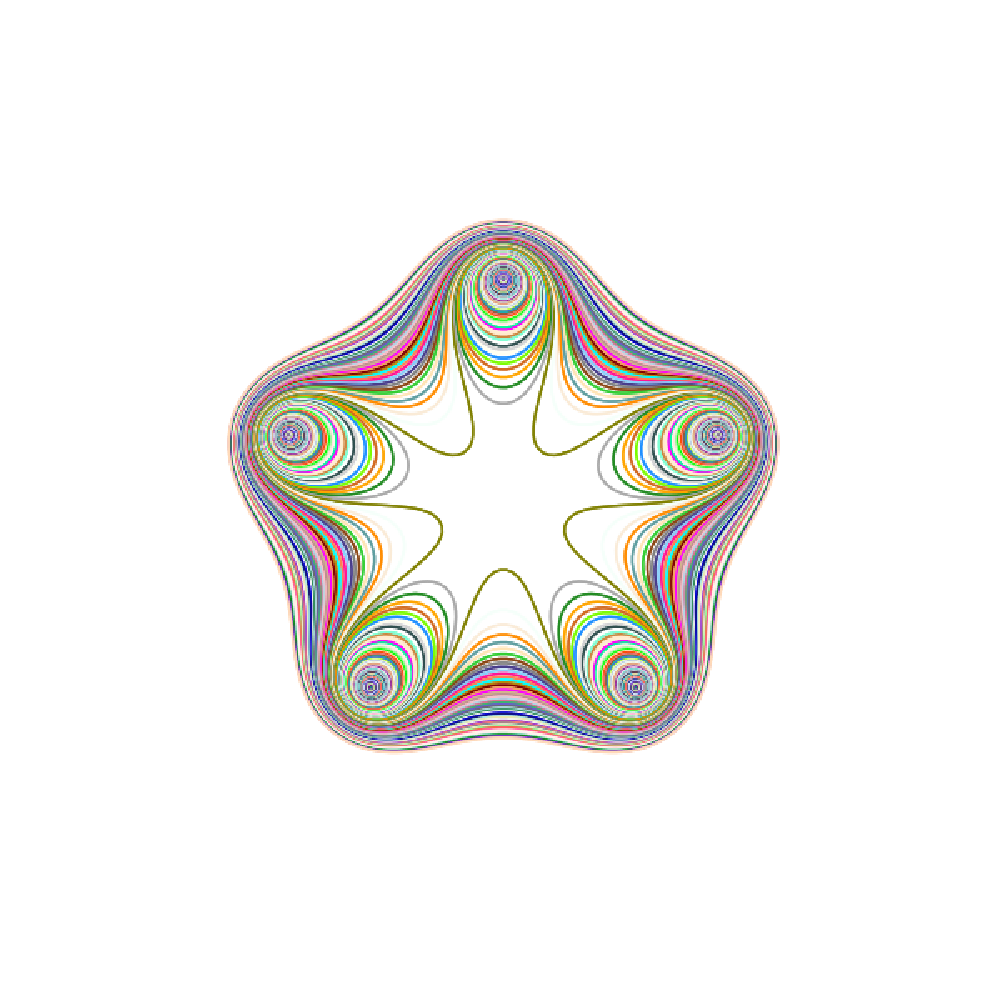
\includegraphics[width=8cm]{cassini5_star.eps}
\caption{}
\label{ }
\end{center}
\end{figure}
\end{exa}
%---- Connected Components ----%
\subsection{Connected Components}
\label{sec-1-6}
\begin{prop}
Let $p_i, (i=1,\cdots,n)$ be distinct points in $\R^D$. Then, for sufficiently small $\delta >0$, the inverse image $C(p_1,\cdots,p_n;\delta)$ have at least $n$ non-intersecting components homeomorphic to $S^{D-1}$ centred at $p_i$.
\end{prop}
\begin{proof}
Let $r_{\min}:= \min_{i,j}\left\{r_{ij}\right\}$, $\delta < \frac{r_{\min}}{2}$ and $B(p_i;\delta):= \defset{x\in \R^D}{\delta >|x-p_i|}$. Let us denote the minimum pair $r_{ab}=r_{\min}$. Then $B(p_i;\delta)\cap B(p_j;\delta) = \emptyset, (\forall i\ne j)$.  We are only interested in their relative positions. So, by multiplying all the coordinates with a suitable constant, we can assume $r_{\min}>2$ so that $\delta <1$. Now, consider the inverse image $C(p_1,\cdots,p_n;\delta)$. Because we have assumed $r_{\min}>2$ and $\delta <1$, for $x\in B(p_a;\delta)$, we have $r_i = |x-p_i|>1, (i\ne a)$. 
\begin{equation}
\label{eq:inequality_radius}
r_a < r_a\prod_{i\ne a}r_i =F(p;x).
\end{equation}
Now, consider a (D-1)-sphere centred at $p_a$ with some radius $\rho < \delta$, $S^{D-1}_{\rho}$. Take a point $y \in S^{D-1}_{\rho}$, then connect it with the centre $p_a$ by line joining them $\overrightarrow{\y \bp_a}$. We want to show that there is a value $\rho_0$ such that for every point $y \in S^{D-1}_{\rho_0}$, there exists a point $\x_0$ on the line $\overrightarrow{\y \bp_a}$ which satisfies $F(\x_0)=\rho_0$. To prove this, let us denote a point $\x$ on the line $\overrightarrow{yp_a}$ by $\x = p_a + \rho \hat{r}$, where $\hat{r} := \frac{\overrightarrow{p_a y}}{|\overrightarrow{p_a y}|}$. Then, 
\begin{equation}
\label{}
F(p;\x(\rho))=\prod_{i=1}^{n} r_i(\rho) = \rho \prod_{i \ne a } (\rho^2 + r^2_{ia} - 2\rho <\mathbf{r}_{ia},\hat{r}>)^{\frac{1}{2}}
\end{equation}
is a strictly incresing funtion of $\rho$ for sufficiently small $\rho$. Indeed
\begin{eqnarray}
\label{}
\frac{d F}{d \rho} &=& \prod_{i \ne a } r_i(\rho) + \rho \sum_{j\ne a } \frac{\rho -  <\mathbf{r}_{ja},\hat{r}>}{r_j(\rho)}\prod_{i \ne a,j } r_i(\rho)\nonumber\\
&=&\prod_{i \ne a } r_i(\rho) \left(1 + \rho\sum_{j\ne a } \frac{ <\rho\hat{r}-\mathbf{r}_{ja},\hat{r}>}{r_j(\rho)^2}\right)\nonumber\\
&=&\prod_{i \ne a } r_i(\rho) \left(1 + \rho\sum_{j\ne a } \frac{ <\mathbf{r}_{j}(\rho),\hat{r}>}{r_j(\rho)^2}\right) \nonumber\\
&=&\prod_{i \ne a } r_i(\rho) \left(1 +  \rho<\sum_{j\ne a }\mathbf{\tilde{r}}_{j}(\rho),\hat{r}> \right)
\end{eqnarray}
Since $\exists M$ such that $\forall \rho \in [0,\delta], |<\sum_{j\ne a }\mathbf{\tilde{r}}_{j}(\rho),\hat{r}>| < M$, the quantity inside the bracket is positive for sufficiently small $\rho$ so that $\frac{d F}{d \rho}>0$. 
\begin{equation}
\label{}
\rho_{min} := \min_{\hat{r}\in S_{D-1}}\left\{\rho: 1 +  \rho<\sum_{j\ne a }\mathbf{\tilde{r}}_{j}(\rho),\hat{r}> \; > 0 \right\}
\end{equation}
Then, by (\ref{eq:inequality_radius}), for each point $\y$ on $S^{D-1}_{\rho_{min}}$
\begin{equation}
\label{}
F(\y) > \rho_{min}
\end{equation}
But, now $F(p;\x(\rho))$ is a strictly increasing function of $\rho$ for any $\hat{r} := \frac{\overrightarrow{p_a y}}{|\overrightarrow{p_a y}|}$, so there exists exactly one $\rho_0$ such that $F(p;\x(\rho_0(\hat{r}))) = \rho_{min}$ for each $\hat{r} \in S^{D-1}$. This means there is a disconnected component of the inverse image of $C(p_1,\cdots,p_n;\rho_{min}) =0$ around $p_a$ homeomorphic to $S^{D-1}$.
\end{proof}
But, the fact is, this is not just good enough to tell you all the components to appear when you vary the value $a$. For $D=3$, Cassinian surfaces with the points located on the unit sphere appear to have an extra component which does'nt contain a focus inside. The central component emerges as a point from the critical point at the origin when $a=1$.
\begin{figure}[H]
%------- TETRAHEDRON -------%
\begin{minipage}{.5\hsize}
\begin{center}
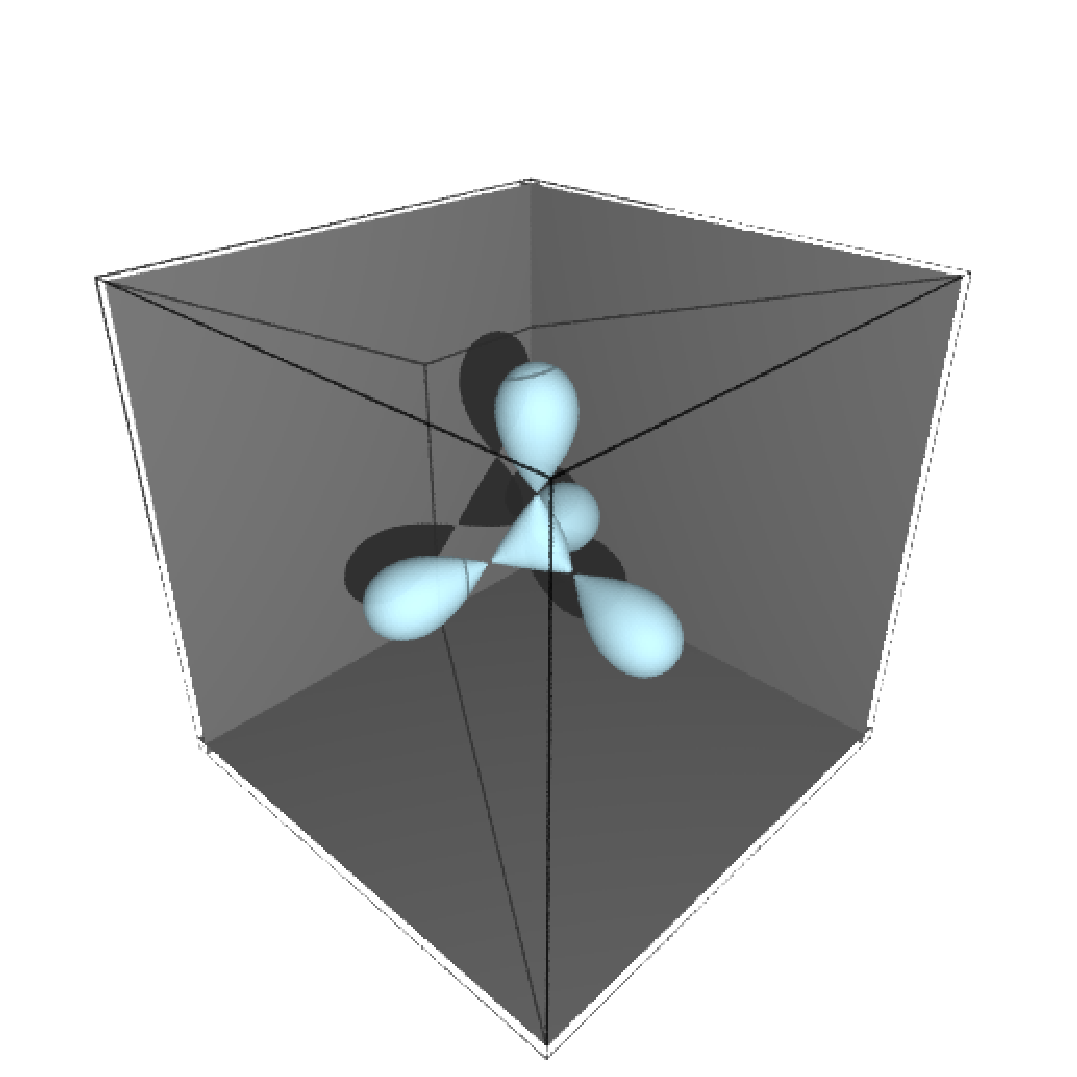
\includegraphics[width=6cm]{tetrahedral_cassini.eps}
\caption{Cassian surface with foci at vertices of a regular tetrahedron.}
\label{}
\end{center}
\end{minipage}
%------- ICOSAHEDRON -------%
\begin{minipage}{0.5\hsize}
\begin{center}
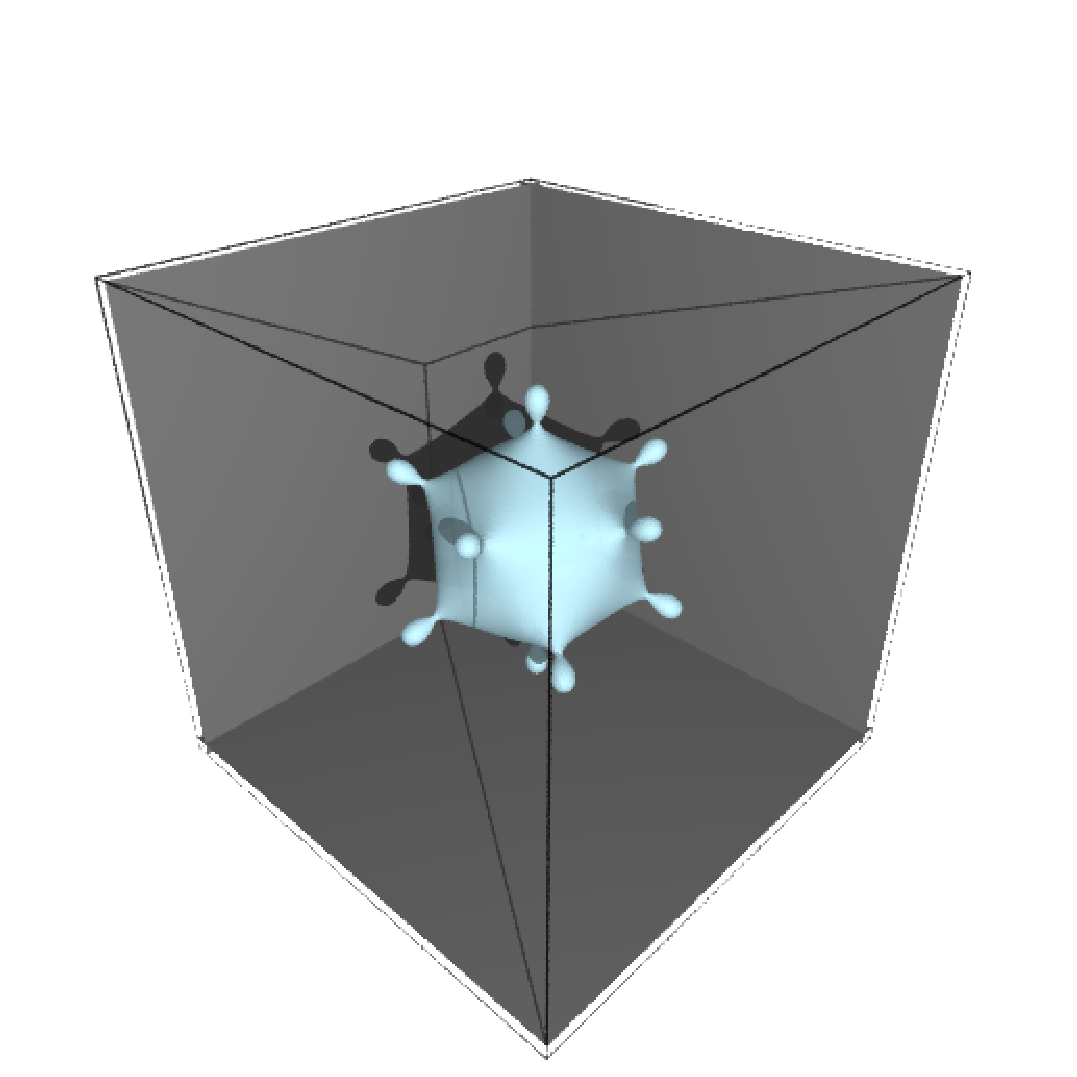
\includegraphics[width=6cm]{icosahedral_cassini.eps}
\caption{Cassian surface with foci at vertices of a regular icosahedron.}
\label{}
\end{center}
\end{minipage}
\end{figure}
%---Self-intersection points ---%
\subsection{Singular points}
\label{sec-1-7}
We want to determine the singular points for the level curve of the function
\begin{equation}
\label{ }
F(x) =  \prod_{i=1}^{n} r_i 
\end{equation}
that is, points $x_0$ with $\partial_{\mu} F(x_0) := \frac{\partial F}{\partial x^{\mu}}(x_0)= 0$ other than foci where total derivatives are not defined. Thus, we will assume that $x_0 \ne p_i$. Then, $r_i \ne 0$, so we can divide the partial derivatives by $r_1 \cdots r_n$, which yields, as a stationary condition
\begin{equation}
\label{eq:stationary}
\frac{1}{2r_1 \cdots r_n}\clmnVsan{\partial_1 F(x_0)}{\vdots}{\partial_D F(x_0)} = \sum_{i=1}^{n} \frac{1}{r_i^2} x_i =0
\end{equation}
where $x_i = x_0-p_i$. By writing the image of $x_i$ under a geometric inversion $\mathcal{I}_{S^{D-1}}$ in unit $D-1$ sphere $S^{D-1}$ centred at $x_0$ as $\tilde{x}_i = \mathcal{I}_{S^{D-1}}(x_i)$, the condition reads as
\begin{equation}
\label{ }
\frac{1}{n}\sum_{i=1}^{n} \tilde{x}_i =0
\end{equation}
which translates geometrically as the barycentre of the polygon whose vertices are the inverse images of the foci must coincide with the centre of the inversion. For $n=2$, it is easy to see that the barycentre is the midpoint of the two foci in any dimension $D$.\\
It can be expressed in terms of mechanical language too. If we consider a set of n points with equal mass located at $p_i$'s, the equation (\ref{eq:stationary}) means that the sum of the centrifugal forces at point $x$ is zero.

Knowing the condition for the self-intersection points, we want to know the barycentre of a polytope in terms of multipolar coordinates. It is actually easy to obtain;
%---PROPOSITION:---%
\begin{prop}
Let $p_1 \cdots, p_n$ be distinct points in $\R^{D}$ and $b:= \frac{1}{n}\sum_{i=1}^{n}p_i$ be the barycentre. Then the multipolar coordinates $r_i := |p_i-b|$ of the barycentre is given by
\begin{equation}
\label{eq:barycentre}
r_i =  \frac{1}{n}\sqrt{ (n-1)\sum_{i\ne j } r_{ij}^2 - \sum_{\substack{j < k \\ j,k \ne i}}r_{jk}^2}
\end{equation}
\end{prop}
%---PROPOSITION:---%
\begin{proof}
\begin{eqnarray}
|p_1-b|^2 & = & \frac{1}{n^2}|(n-1)p_1-(p_2 + \cdots + p_n)|^2 \nonumber\\
 & = & \frac{1}{n^2}|\textbf r _{12} + \cdots + \textbf r_{1n}|^2 \nonumber\\
 &=& \frac{1}{n^2}\left\{\sum_{1\ne j} r_{1j}^2 + 2\sum_{\substack{j < k \\ j,k \ne 1}}\textbf r_{1j}\cdot \textbf r_{1k}\right\}
\end{eqnarray}
where $\textbf r_{ij} : = p_i - p_j$ and $r_{ij} = |\textbf r_{ij}|$. Then, from the cosine rule, $2\textbf r_{1j}\cdot \textbf r_{1k} = r_{1j}^2 + r_{1k}^2 - r_{jk}^2$,
\begin{eqnarray}
|p_1-b|^2 &=& \frac{1}{n^2}\left\{\sum_{1\ne j} r_{1j}^2 + \sum_{\substack{j < k \\ j,k \ne 1}}r_{1j}^2 + r_{1k}^2 - r_{jk}^2\right\} \nonumber\\
&=& \frac{1}{n^2}\left\{\sum_{1\ne j} r_{1j}^2 + \sum_{\substack{j < k \\ j,k \ne 1}}(r_{1j}^2 + r_{1k}^2 )-  \sum_{\substack{j < k \\ j,k \ne 1}} r_{jk}^2\right\} \nonumber\\
&=& \frac{1}{n^2}\left\{\sum_{1\ne j} r_{1j}^2 +(n-2) \sum_{1\ne j}r_{1j}^2 -  \sum_{\substack{j < k \\ j,k \ne 1}} r_{jk}^2\right\} \nonumber\\
&=& \frac{1}{n^2}\left\{(n-1) \sum_{1\ne j}r_{1j}^2 -  \sum_{\substack{j < k \\ j,k \ne 1}} r_{jk}^2\right\} \nonumber
\end{eqnarray}
\end{proof}
%---END OF PROOF---%
A way to remember (\ref{eq:barycentre}) is that the first sum inside the square root consists of edges connected to $p_i$ and the second sum contains those not connected to $p_i$. Let us denote the barycentre determined by the data $\{r_{ij}\}_{1\le i < j\le n}$, the distances between points $p_i$'s as
\begin{equation}
\label{ }
Bary(r_{ij}) := r_1 : \cdots : r_n  .
\end{equation}
Then the explicit condition for the stationary points is
\begin{equation}
\label{ }
Bary\left(\frac{r_{ij}}{r_i r_j}\right) := \frac{1}{r_1} : \cdots : \frac{1}{r_n}  .
\end{equation}
By substituting $u_i = \frac{1}{r_i^2}$, and writing $R_{ij} := r^2_{ij}$
\begin{equation}
\label{}
n^2 u_i =   (n-1)\sum_{i\ne j } R_{ij}u_i u_j - \sum_{\substack{j < k \\ j,k \ne i}}R_{jk}u_j u_k
\end{equation}
Hence
\begin{equation}
\label{}
\left\{ (n-1)\sum_{i\ne j } R_{ij} u_j - n^2 \right\} u_i =     \sum_{\substack{j < k \\ j,k \ne i}}R_{jk}u_j u_k
\end{equation}
If the quatity inside the bracket on the l.h.s. is non-zero for all $i$, we can obtain an equation for $u_i$ of degree $n+1$, by eliminating other indices,
\begin{equation}
\label{}
A_{n+1}(R;i)u_i^{n+1} + \cdots +A_{1}(R;i)u_i + A_0(R;i) = 0.
\end{equation}
Together with $n$ equations of the above form, we also have combpatibility conditions. And by solving the system of equations or equations and inequalities, we can determine the polar coordinates of the singular points and hence the values $a^2$ at which they appear.\\
UNSOLVED:Can we know the number of the positive roots to this equation?\\
The use of Groebner basis may solve the problem.
 An observation tells us that it seems that there $n-1$ solutions when all the foci are in the same 2-D plane and $n$ solutions when $n\ge 4$ and all the foci are in the same 3-D hyperplane. What about for $n \ge 5$ when all the foci are in the same 4-D hyperplane?

In $D=2$ case, we can use complex numbers to obtain the same result. For that end, let us consider the polynomial function $P(z)$
\begin{equation}
\label{}
w = P(z) = (z-p_1)(z-p_2)\cdots(z-p_n)
\end{equation}
Then, Cassinian curves are defined to be the set
\begin{equation}
\label{ }
C(P,a) := \left\{ z \in \C | \;|P(z)| = a \right\}.
\end{equation}
It can also be seen as the inverse image of a circle of radius $a$ centred at the origin. And the singular points are simply the zeros of the derivative $\frac{dP}{dz}$: that is
\begin{equation}
\label{ }
\frac{dP}{dz} = \sum_{i=1}^{n} (z-p_1)\overset{i}{\breve{\cdots} }(z-p_n) = 0
\end{equation}
where $\overset{i}{\breve{\cdots} }$ means $i$-th product is omitted. It is obvious $\frac{dP}{dz}(p_i) \ne 0$ for all $p_i$. So, we can assume $z \ne p_i$ and have
\begin{equation}
\label{ }
\sum_{i=1}^{n} \frac{1}{z-p_1} = 0
\end{equation}
which is the same as the geometric inversion except that the orientation is reversed in this case.
\subsubsection{Some explicit calculations}
\label{sec-1-7-1}
Let us consider the case $n=3$, where we can work again in the 2 dimensional plane which contains the foci. Then, for a triangle $\triangle ABC$ with sides' lengths $(a,b,c)$ and a point on the plane, let us call the triplet $x:y:z$ of the distances $AP$, $BP$ and $CP$ respectively, the tripolar coordinates. Then the tripolar coordinates of the barycentre of $\triangle ABC$ is given by
\begin{equation}
\label{ }
Bary(a,b,c) : = \frac{1}{3}\sqrt{2(b^2 + c^2)-a^2} : \frac{1}{3}\sqrt{2(c^2 + a^2)-b^2} : \frac{1}{3}\sqrt{2(a^2 + b^2)-c^2} 
\end{equation}
Notice that $Bary(ka,kb,kc) = k\; Bary(a,b,c)$. Now, from inversion geometry, the lengths $(a^{\prime},b^{\prime},c^{\prime})$ of the sides of $\triangle \tilde{A}\tilde{B}\tilde{C}$ are given by
\begin{equation}
\label{ }
(a^{\prime},b^{\prime},c^{\prime}) = \left( \frac{a}{yz},\frac{b}{zx}, \frac{c}{xy} \right).
\end{equation}
Therefore, the stationary condition now reads as
\begin{equation}
\label{ }
\frac{1}{x}:\frac{1}{y}:\frac{1}{z} = Bary(a^{\prime},b^{\prime},c^{\prime}) = Bary\left( \frac{a}{yz},\frac{b}{zx}, \frac{c}{xy} \right).
\end{equation}
multiplying both sides by $xyz$, we get
\begin{equation}
\label{ }
yz:zx:xy = Bary(ax,by,cz).
\end{equation}
The solutions for these equations should give us the stationary points.
%---FIGURE:Singular points for triangle ---%
\begin{figure}[H]
\begin{center}
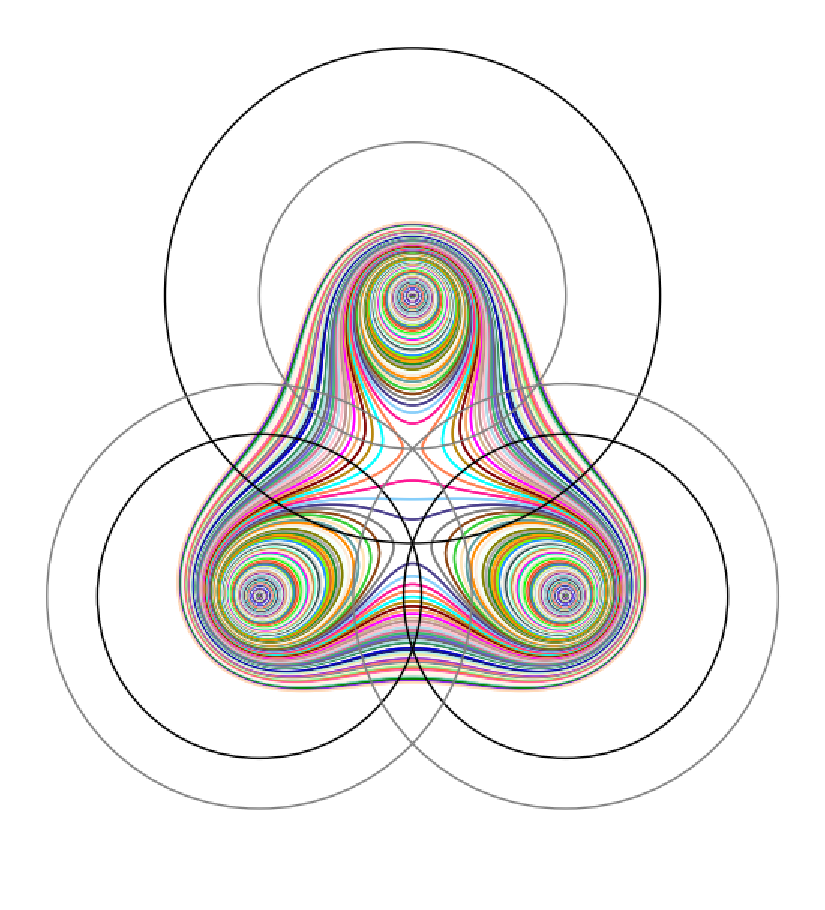
\includegraphics[width=6cm]{tripolar_singular_points.eps}
\caption{The position of the singular points are calculated in tripolar coordinates and then plotted as the points of intersections of three circles centred at the foci. There are two such singular points where three circles of the same colour meet.}
\label{ }
\end{center}
\end{figure}
\section{Surfaces of Arbitrary Genus Constructed from Generalised Cassinian Curves}
\label{sec-2}
Refinement of a statement made in a problem in the book (Morris \cite{Hirsch} p28. problem 12)
\begin{thm}
 If a curve defined by $F(x,y) = 0$, where $F:\R^2 \rightarrow \R$, is closed and has $n-1$ crossings, then we can construct a genus $n$ surface in $\R^3$ by setting
\begin{equation}
\label{ }
F(x,y)^2 - ( r^2 - z^2) = 0 
\end{equation}
for some $r$.
\end{thm}
\begin{proof}
 First, we want to show for some $r > 0$, if $F^{-1}(r)$ is connected regular (a Jordan curve) then $F^{-1}(-r)$ consist of $n$ compnents (the case $F^{-1}(-r)$ is connected is really the same if set $F' = -F$). Then, from the factorisation
\begin{equation}
\label{ }
(F(x,y) + \sqrt{r^2-z^2})(F(x,y) - \sqrt{r^2-z^2}) = 0
\end{equation}
 We can see that the level cruves at $z=\pm r$ have $n-1$ crossings and for $z \in (-r,r)$ split into the outer curve $F^{-1}(\sqrt{r^2-z^2})$ and the inner $n$ curves $F^{-1}(-\sqrt{r^2-z^2})$.
\end{proof}
CONSIDERATION: Suppose \$F:\R$^{\text{2}}$ $\rightarrow$ \R \$ has $n-1$ crossings (the number of critical points may be less than the number of crossings), say $\{p_{i}\}$, and every inverse image $F^{-1}(a)$ for $a\in F(\R^2)$ is closed and denote $z_i=F(p_i)$ and set $M:= \max\{z_i\}$ and \$ m :=$\min$ \{z$_{\text{i$\backslash$}}$\}\$. For $a>M$, $F^{-1}(a)$ is connected(?),and does $F^{-1}(a<m)$ have $n$ components? ANSWER: In general, $F^{-1}(a>M)$ is not connected, but if $F^{-1}(a)$ is connected for $a>M$, then .\\
Question: If $F^{-1}(a>M)$ is connected , by suitably adjusting the constant, we can assume $M=0$. If we pick up a $r< m-M, \; r \in F(\R^2)$ , then a surface defined by
\begin{equation}
\label{ }
F(x,y)^2 + (r^2 - z^2) = 0
\end{equation}
has genus $n$?
\%---SUBSESCTION: EXAMPLES OF COOKIES
\subsection{Examples of Cassinian Cookies}
\label{sec-2-1}
\begin{figure}[H]
%------- Omusubi 4-Cassinian -------%
\begin{minipage}{0.5\hsize}
\begin{center}
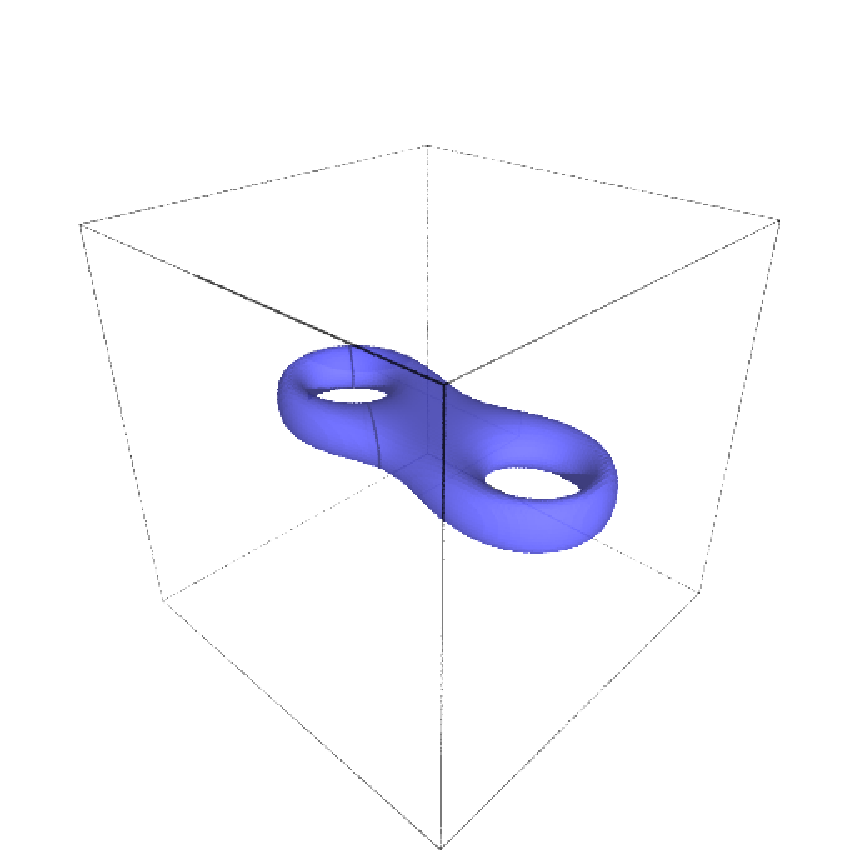
\includegraphics[width=6cm]{cookie2.eps}
\caption{}
\label{ }
\end{center}
\end{minipage}
%------- Aligned 4-Cassinian -------%
\begin{minipage}{0.5\hsize}
\begin{center}
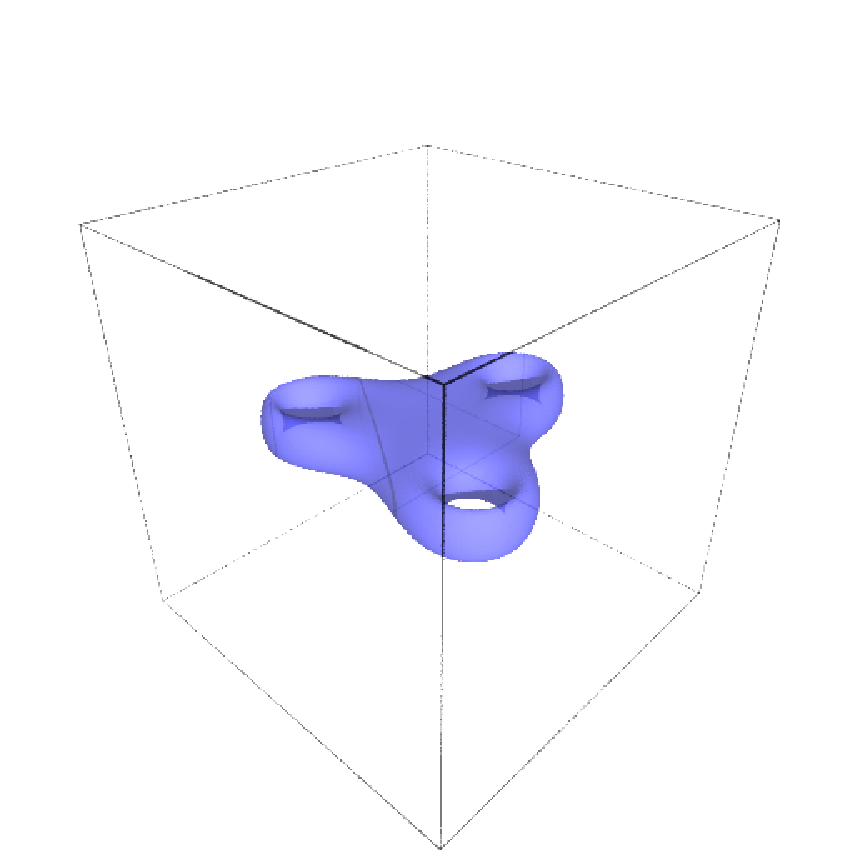
\includegraphics[width=6cm]{cookie3_omusubi.eps}
\caption{}
\label{ }
\end{center}
\end{minipage}
\end{figure}
%------- Clover 4-Cassinian -------%
\begin{figure}[H]
\begin{center}
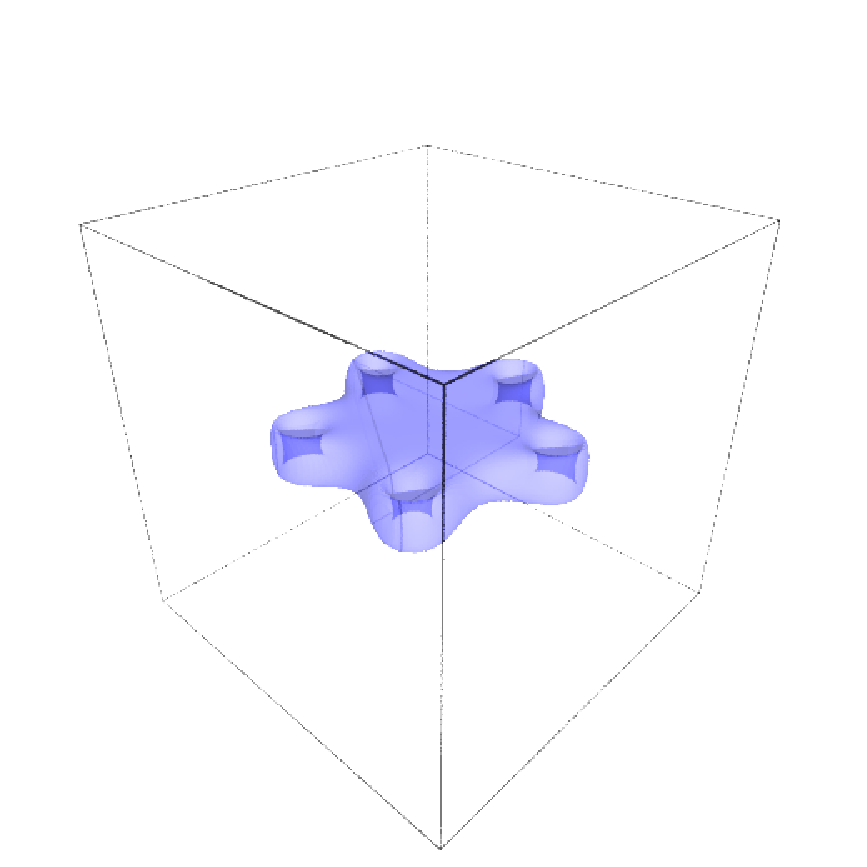
\includegraphics[width=6cm]{cookie5_star.eps}
\caption{}
\label{}
\end{center}
\end{figure}
%---SECTION: Cassinian cookies in 4D---% 
\section{Cassinian Cookies in 4D}
\label{sec-3}
\begin{equation}
\label{}
F(x^1,x^2,x^3)^2 - ( r^2 - (x^4)^2) = 0 
\end{equation}
When $n=2$, we can assume that $p_1 = (p,0,0)$ and $p_2 = (-p,0,0)$ without loss of generality. 
$r_1= \sqrt{(x^1-p)^2 + (x^2)^2 + (x^3)^2}= \sqrt{(x^1-p)^2 + R^2}$, $r_2 = \sqrt{(x^1+p)^2 + (x^2)^2 +  (x^3)^2}= \sqrt{(x^1+p)^2 + R^2}$ where $R^2 = (x^2)^2 + (x^3)^2$
\begin{equation}
\label{}
F(x^1,x^2,x^3)= r_1r_2 -a^2
\end{equation}

\section{The Limit $n \to \infty$ with Points on Unit Circle}
\label{sec-4}
Consider points of regular $n$-gon $\{p_i=(\cos{\theta_i,\sin{\theta_i}})| \theta_i = \frac{2i\pi}{n}, \; i = 0,\cdots,n-1\}$. And set
\begin{equation}
\label{ }
F_n(x) := \prod_{i=0}^{n-1}|x-p_i|
\end{equation}
What will happen when we take the limit $n \to \infty$?
%-------- APPENDICES -----------%
\appendix
\section{Compatibility Conditions For A Triangle}
\label{sec-5}
Use the cosine rule for each side:
\begin{eqnarray}
r_{12}^2 & = & r_1^2 + r_2^2 - 2r_1r_2\cos{\alpha} \\
r_{31}^2 & = & r_3^2 + r_1^2 - 2r_3r_1\cos{\beta} \\
r_{23}^2 & = & r_2^2 + r_3^2 - 2r_2r_3\cos{\gamma} 
\end{eqnarray}
and also the fact that the total angle is $\alpha + \beta +\gamma = 2\pi$ so
\begin{equation}
\label{ }
\cos{(\alpha + \beta +\gamma)} = 1.
\end{equation}
By addition theorem, this implies
\begin{equation}
\label{eq:cosine_for_three}
1= \cos^2{\alpha} + \cos^2{\beta} + \cos^2{\gamma} -2 \cos{\alpha} \cos{\beta} \cos{\gamma}.
\end{equation}
Equating the first three expressions to cosines and then substituing them into (\ref{eq:cosine_for_three}) yields the compatibility condition for triangles.
\section{Solid Angles and Compatibility Conditions For A Tetrahedron}
\label{sec-6}
The spherical cosine rule:
consider a triangle on a sphere i.e. a region on a sphere bounded by three distinct greater circles. Let us denote the length of the three sides by $\alpha$, $\beta$ and $\gamma$, and the corresponding opposite dihedral angles by $A$, $B$ and $C$.
\begin{equation}
\label{ }
\cos{C} = \frac{\cos{\gamma} - \cos{\alpha}\cos{\beta} }{\sin{\alpha}\sin{\beta}}
\end{equation}
Let us denote the solid angles above respectively by $\Theta_{ABC}$, $\Theta_{ACD}$, $\Theta_{ABD}$ and $\Theta_{BCD}$. And let us denote by, for example, $\theta_{BAC}$ the dihedral angle subtended by the greater circles on the unit sphere centred at $x$, which pass through the projected points of $A$, $B$ and $C$. Then it follows that 
\begin{eqnarray}
\Theta_{ABC} & = & \theta_{BAC} + \theta_{ACB} + \theta_{ABC} - \pi \\
\Theta_{ACD} & = & \theta_{ACD} + \theta_{CDA} + \theta_{CAD} - \pi \\
\Theta_{ABD} & = & \theta_{ABD} + \theta_{BDA} + \theta_{BAD} - \pi \\
\Theta_{BCD} & = & \theta_{BCD} + \theta_{CBD} + \theta_{BDC} - \pi 
\end{eqnarray}
And then the compatibility condition for the tetrahedron is
\begin{equation}
\label{ }
\Theta_{ABC} + \Theta_{ABD} + \Theta_{ACD} + \Theta_{BCD} = 4\pi
\end{equation}
But we also have $\theta_{BAC} + \theta_{CAD} + \theta_{DAB} = 2\pi$ for each vertices.
%-----------  Bibliography ----------------
\begin{thebibliography}{10}
\bibitem{Hirsch}
  Morris W. Hirsch, Differential Topology, Springer Verlag, 1976
\bibitem{Cayley}
  A. Cayley, The Cambridge Mathematical Journal, vol. II, 267-271
\end{thebibliography}
% Emacs 25.3.2 (Org mode 8.2.10)
\end{document}